\documentclass[12pt,a4paper]{scrartcl}
\usepackage[margin=2.2cm]{geometry}
\usepackage[utf8]{inputenc}
\usepackage{slovak}
\usepackage{float}
\usepackage{graphicx}
\usepackage{hyperref}
\begin{document}
\title{Turistický denník}
\subtitle{Špecifikácia na Tvorbu internetových aplikácií}
\author{Ladislav Bačo}
\maketitle
\bigskip
\abstract{
Online systém na zaznamenávanie turistických výletov a ich zdieľanie s priateľmi.
}

\vfil
\begin{center}
	\begin{tabular}{|c|c|}
		\hline
		\bf Špecifikácia & \bf Dátum \\
		\hline
		Verzia 1.0 & 18.3.2014 \\
		\hline
		Verzia 2.0 & 21.3.2014 \\
		\hline
	\end{tabular}
\end{center}
\thispagestyle{empty}

\newpage
\section{Úvod}
Aplikácia je určená na zaznamenávanie absolvovaných výletov, prezeranie štatistík a zdieľanie výletov s priateľmi. Registrovaní užíavtelia môžu vytvárať záznamy o svojich výletoch, nahrávať súbory s gpx logmi prejdenej trasy, zobrazovať trasu výletov na mape spolu s výškovým profilom (z gpx logu). K jednotlivým výletom je možné pridať textový popis a fotky, zobraziť základné štatistiky o výlete (prejdená vzdialenosť, prevýšenie, trvanie výletu, priemerná rýchlosť). Ďalej majú užívatelia možnosť zdieľať svoje výlety s priateľmi (resp. skupinami priateľov) registrovanými na stránke a komentovať výlety zdieľané s nimi.

\section{Definícia pojmov}
\begin{itemize}
	\item{\bf Neprihlásený užívateľ:} návštevník stánky, ktorý nie je zaregistrovaný alebo aktuálne nie je prihlásený
	\item{\bf Užívateľ:} registrovaný návštevník stránky, ktorý je aktuálne prihlásený
	\item{\bf Administrátor:} prihlásený návštevník stránky so špeciálnymi právami správcu
	\item{\bf Blokovaný užívateľ:} užívateľ, ktorý sa nejakým spôsobom previnil a administrátor mu kvôli tomu zablokoval možnosť prihláseniť sa
	\item{\bf Skupina:} množina registrovaných užívateľov (aj neprihlásených), ktorú vytvoril a pomenoval jeden konkrétny užívateľ a s ktorou môže zdieľať svoje výlety
	\item{\bf Výlet:} záznam o turistickej (prípadne cykloturistickej) aktivite užívateľa obsahujúci informácie o prejdenej trase a prípadne aj fotky
	\item{\bf Zdieľanie výletu:} poskytovanie možnosti zobraziť a komentovať výlet ďalším užívateľom 
	\item{\bf Komentár:} textová správa asociovaná s výletom, v ktorej môžu užívatelia vyjadriť svoj názor na výlet
\end{itemize}

\section{Prípady použitia}
\subsection{Správa užívateľov}
\begin{figure}[H]
	\centering
	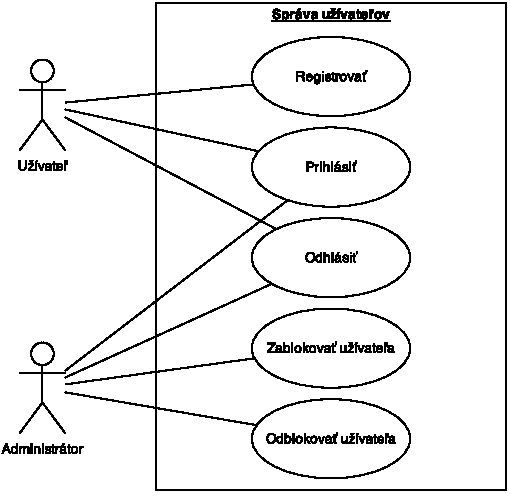
\includegraphics{use_case/turistika_sprava_uzivatelov.pdf}
	\caption{Správa užívateľov}
\end{figure}

Neprihlásení užívatelia sa na stránke môžu zaregistrovať a prihlásiť (ak sa predtým zaregistrovali). Prihlásený užívateľ sa môže odhlásiť. Administrátor má okrem prihlásenia a odhlásenia možnosť zablokovať užívateľov, ktorí sa nejakým spôsobom previnili. V prípade zablokovania bude blokovaný užívateľ informovaný mailom. Po prípadnej mailovej konverzácii môže administrátor blokovaného užívateľa odblokovať.

\subsection{Správa skupín}
\begin{figure}[H]
	\centering
	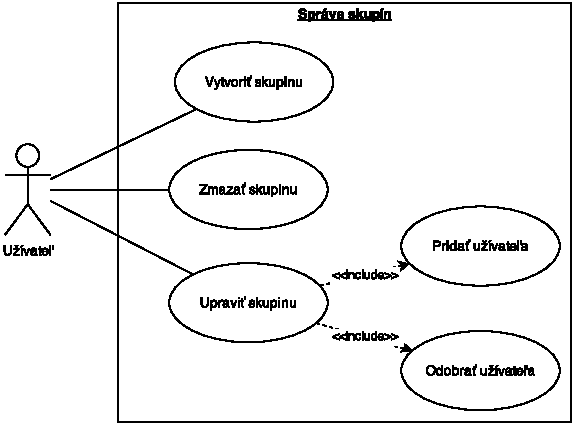
\includegraphics{use_case/turistika_sprava_skupin.pdf}
	\caption{Správa skupín}
\end{figure}

Užívateľ si môže vytvoriť vlastné skupiny užívateľov (napr. rodina, priatelia, spolužiaci), s ktorými potom môže jednoduchšie zdieľať výlety. Vlastné vytvorené skupiny môže užívateľ upravovať (pridať a odobrať užívateľa) alebo ich zmazať, ak už danú skupinu nepotrebuje.

\subsection{Správa výletov}
\begin{figure}[H]
	\centering
	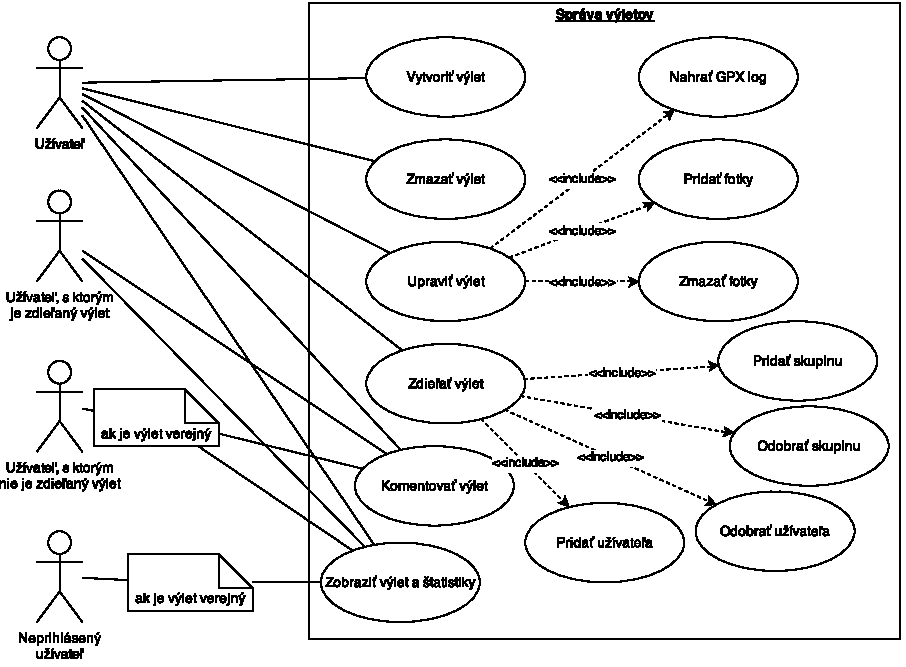
\includegraphics{use_case/turistika_sprava_vyletov.pdf}
	\caption{Správa výletov}
\end{figure}

Užívateľ môže vytvárať, mazať a upravovať svoje výlety. Každý výlet môže mať nejaký textový popis a záznam prejdenej trasy v GPX formáte, tiež sa dajú pridať k výletu aj fotky (a prípadne aj neskôr odstrániť). Každý výlet môže jeho vlastník (užívateľ, ktorý výlet vytvoril) zdieľať buď s vybranými svojimi skupinami alebo jednotlivými inými registrovanými užívateľmi aplikácie, prípadne nastaviť výlet ako verejný. Vlastník a užívatelia, s ktorými je výlet zdieľaný, môžu zobraziť výlet, jeho podrobnosti, fotky a štatistiky a tiež môžu k výletu písať komentáre. Ak je výlet verejný, písať komentáre môže hocijaký prihlásený užívateľ a zobraziť výlet môže aj neprihlásený návštevník stránky.

\section{Návrh databázy}

\begin{figure}[H]
	\centering
	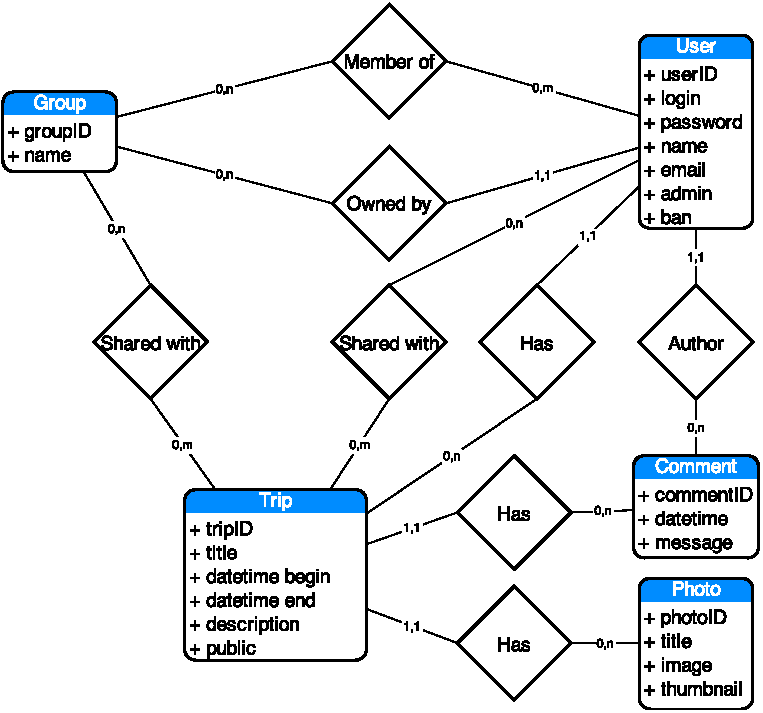
\includegraphics{use_case/turistika_er_diagram.pdf}
	\caption{ER diagram}
\end{figure}

Databáza bude obsahovať 5 základných entít: User, Group, Trip, Comment a Photo. Každej tejto entite bude zodpovedať jedna tabuľka. V databáze budú aj ďalšie tabuľky pre uloženie many-to-many relácii medzi uvedenými entitami: MemberOf(Group, User), SharedWithGroup(Trip, Group), SharedWithUser(Trip, User). Posledné dve tabuľky sa prípadne dajú zlúčiť do jednej SharedWith(Trip, SubjectID, Type) použitím flagu Type, ktorý určí, či ide o prepojenie výletu a užívateľa, alebo výletu a skupiny. Relácie one-to-many a many-to-one môžu byť implementované pridaním ďalších atribútov do entít.

Databáza teda bude pozostávať z týchto tabuliek:
\begin{itemize}
	\item{\bf User:} userID, login, password (hash), name, email, admin (bool flag), ban (bool flag)
	\item{\bf Group:} groupID, name, owner (userID)
	\item{\bf Trip:} tripID, title, begin, end, description, public (bool flag), owner (userID)
	\item{\bf Comment:} commentID, datetime, message, author (userID), trip (tripID)
	\item{\bf Photo:} photoID, title, image, thumbnail, trip (tripID)
	\item{\bf MemberOf:} groupID, userID
	\item{\bf SharedWith:} tripID, whoID (userID alebo groupID), type (group alebo user)
\end{itemize}

\section{Technológie}
Aplikácia bude naprogramovaná vo frameworku Django v jazyku Python, ako databáza bude použitá MySQL. V klientskej časti plánujem využívať jQuery, jQuery Mobile, na zobrazovanie výškových profilov Flot, na zobrazovanie máp OpenLayers a mapové podklady z OpenStreetMap, prípadne Map1.eu a Freemap.sk.
Online verzia bude pravdepodobne hostovaná na OpenShift (\href{http://turistika-cestovatel.rhcloud.com}{turistika-cestovatel.rhcloud.com}), čo je online cloudová aplikačná platforma od Red Hatu.

Doteraz nemám s Djangom žiadne skúsenosti, bude to moja prvá aplikácia a pri jej vývoji sa plánujem naučiť pracovať s týmto frameworkom. Ak by sa po prvých dvoch týždňoch ukázali nejaké veľké problémy, skúsim narýchlo nejaký iný Python framework, v prípade núdze použijem PHP.

Aplikácia bude podporovať prehliadače Mozilla Firefox 20.0 a novšie, Google Chrome 27.0 a novšie a Opera 12.16 pre Linux. A možno aj Internet Explorer (verzia na školských počítačoch), ak bude čas otestovať to a zapracovať na tom.

\section{Časový harmonogram}
\begin{itemize}
	\item{\bf 17.3.-23.3.2014} Špecifikácia, rozbehanie frameworku Django a online hostingu, pokusná Hello world aplikácia (\href{http://hello-cestovatel.rhcloud.com}{hello-cestovatel.rhcloud.com})
	\item{\bf 24.3.-30.3.2014} Správa užívateľov
	\item{\bf 31.3.-6.4.2014} Správa skupín
	\item{\bf 7.4.-13.4.2014} Správa výletov: vytváranie, mazanie, úprava výletov (GPX logy)
	\item{\bf 14.4.-20.4.2014} Správa výletov: zdieľanie výletov, štatistiky, beta verzia
	\item{\bf 21.4.-27.4.2014} Správa výletov: úprava výletov (fotky), komentáre
	\item{\bf 28.4.-4.5.2014} Dokončovanie predchádzajúcich etáp
	\item{\bf 5.5.-11.5.2014} Grafická úprava, design
	\item{\bf 12.5.-18.5.2014} Dolaďovanie posledných detailov, prípadná podpora Internet Exploreru, finálna verzia
\end{itemize}

\section{Budúca práca}

Vytvoriť mobilnú aplikáciu so schopnosťou odosielať aktuálnu polohu (alebo dočasne použiť Osmand), pridať užívateľom možnosť zdieľať svoju aktuálnu polohu, upravovať trasu výletov na základe aktuálnej polohy.

\end{document}
